% Reference https://www.youtube.com/watch?v=Boltwen-g1g&ab_channel=ChandraHas

\documentclass[11pt,a4paper]{article}

% General
\usepackage[margin=1in]{geometry}
\usepackage[sort&compress,square,numbers]{natbib}
\usepackage{amsmath}
\usepackage{lipsum,times,graphicx,hyperref,cleveref}
\hypersetup{nolinks=true}
\usepackage[labelfont=bf]{caption}
\usepackage{amssymb}

\usepackage{physics}
\usepackage{siunitx}
\usepackage{listings}
\usepackage{array,multirow}

% More graphics
\usepackage[label font={bf, normalsize}]{subfig}
\renewcommand{\thesubfigure}{\Alph{subfigure}}
\usepackage{caption}
\captionsetup{font=normal}
\usepackage{floatrow}
\floatsetup[figure]{subcapbesideposition=top}
\floatsetup[table]{style=plaintop}

\usepackage{titling}
\renewcommand\maketitlehooka{\null\mbox{}\vfill}
\renewcommand\maketitlehookd{\vfill\null}

\usepackage{xr}
\externaldocument[main-]{main}
\externaldocument[fig-]{figures}

\title{\vspace{-5cm} {Supplementary material}\\[5mm] 
\textbf{Behavior of weakly adsorbing protein impurities in flow-through ion-exchange chromatography}}
 
\author{Chase E. Herman, Xuankuo Xu, Steven J. Traylor, Sanchayita Ghose, \and Zheng Jian Li, and Abraham M. Lenhoff}

\date{}

%\renewcommand{\figurename}{Fig.}
\renewcommand{\baselinestretch}{1.33} 
\renewcommand{\thepage}{S\arabic{page}}
\renewcommand{\thetable}{S\arabic{table}}
\renewcommand{\thefigure}{S\arabic{figure}}
\renewcommand{\theequation}{S\arabic{equation}}
%==============================Content=========================
\begin{document}

\begin{titlingpage}
\maketitle
\end{titlingpage}

\begin{figure}[H]
    \centering
    \sidesubfloat[]{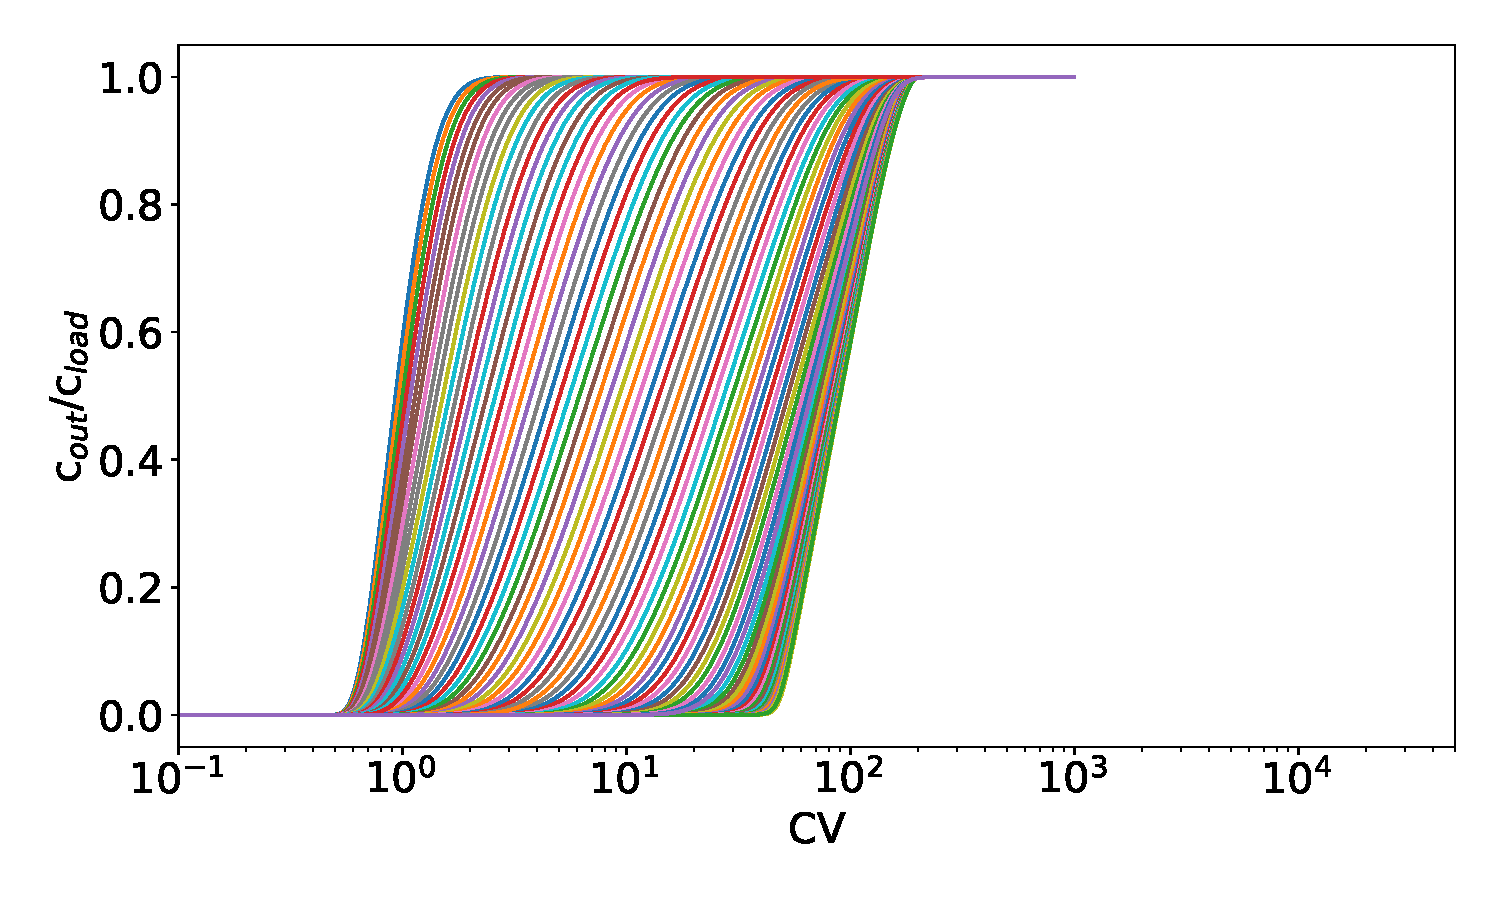
\includegraphics[width=0.75\textwidth]{figure_s1a}}
    \\
    \sidesubfloat[]{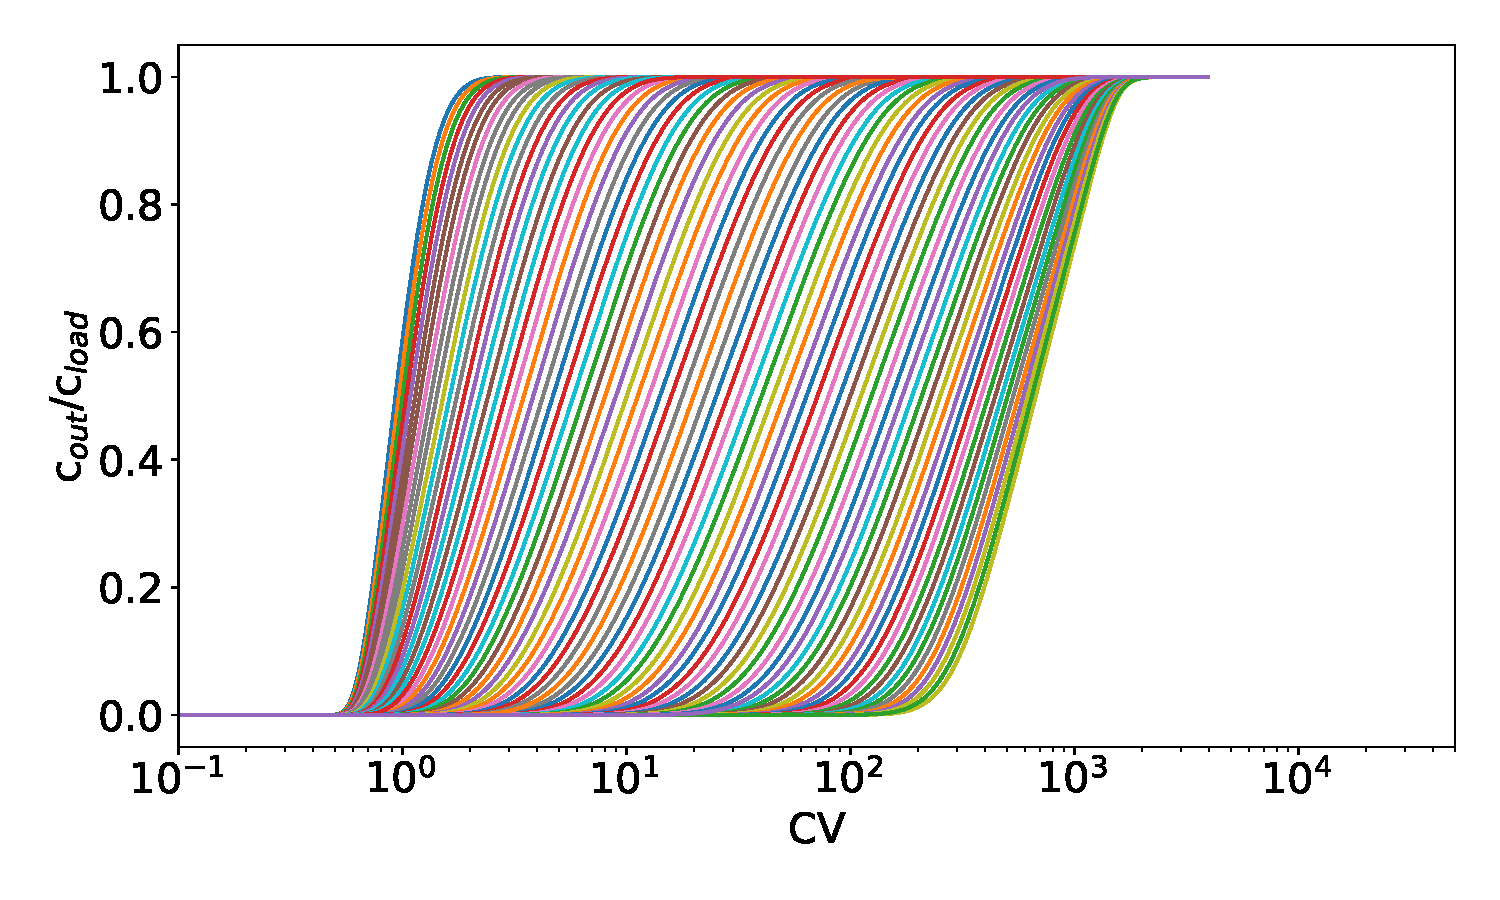
\includegraphics[width=0.75\textwidth]{figure_s1b}}
    \\
    \sidesubfloat[]{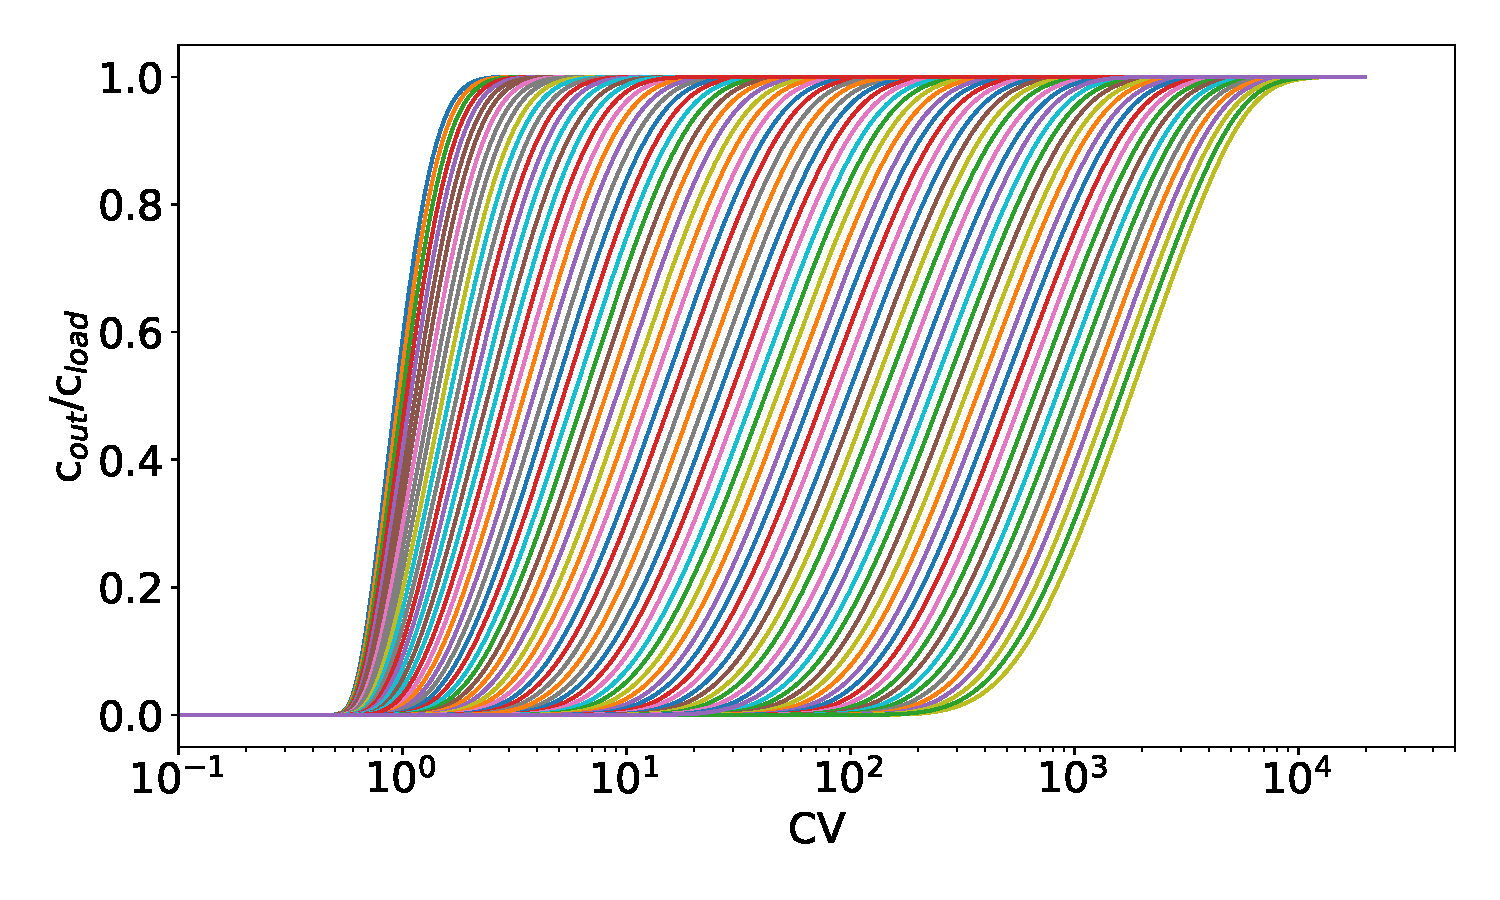
\includegraphics[width=0.75\textwidth]{figure_s1c}}
    
    \caption{Breakthrough profiles from a simulation of solute loading at (A) 1 mg/ml, (B) 100 $\mu$g/ml, and (C) 10 $\mu$g/ml. Lines correspond to simulations with different $K_{eq}$, which increases by 4 orders of magnitude from left to right. Note that $q_{max}$ was fixed at 100 mg/ml of packed column for all simulations, and the abscissa is on a logarithmic scale.}
    
    \label{fig:exploratory breakthrough curves - other concentrations}
\end{figure}

\begin{figure}[H]
    \centering
    \vspace{-5.2cm}
    \makebox[\textwidth][c]{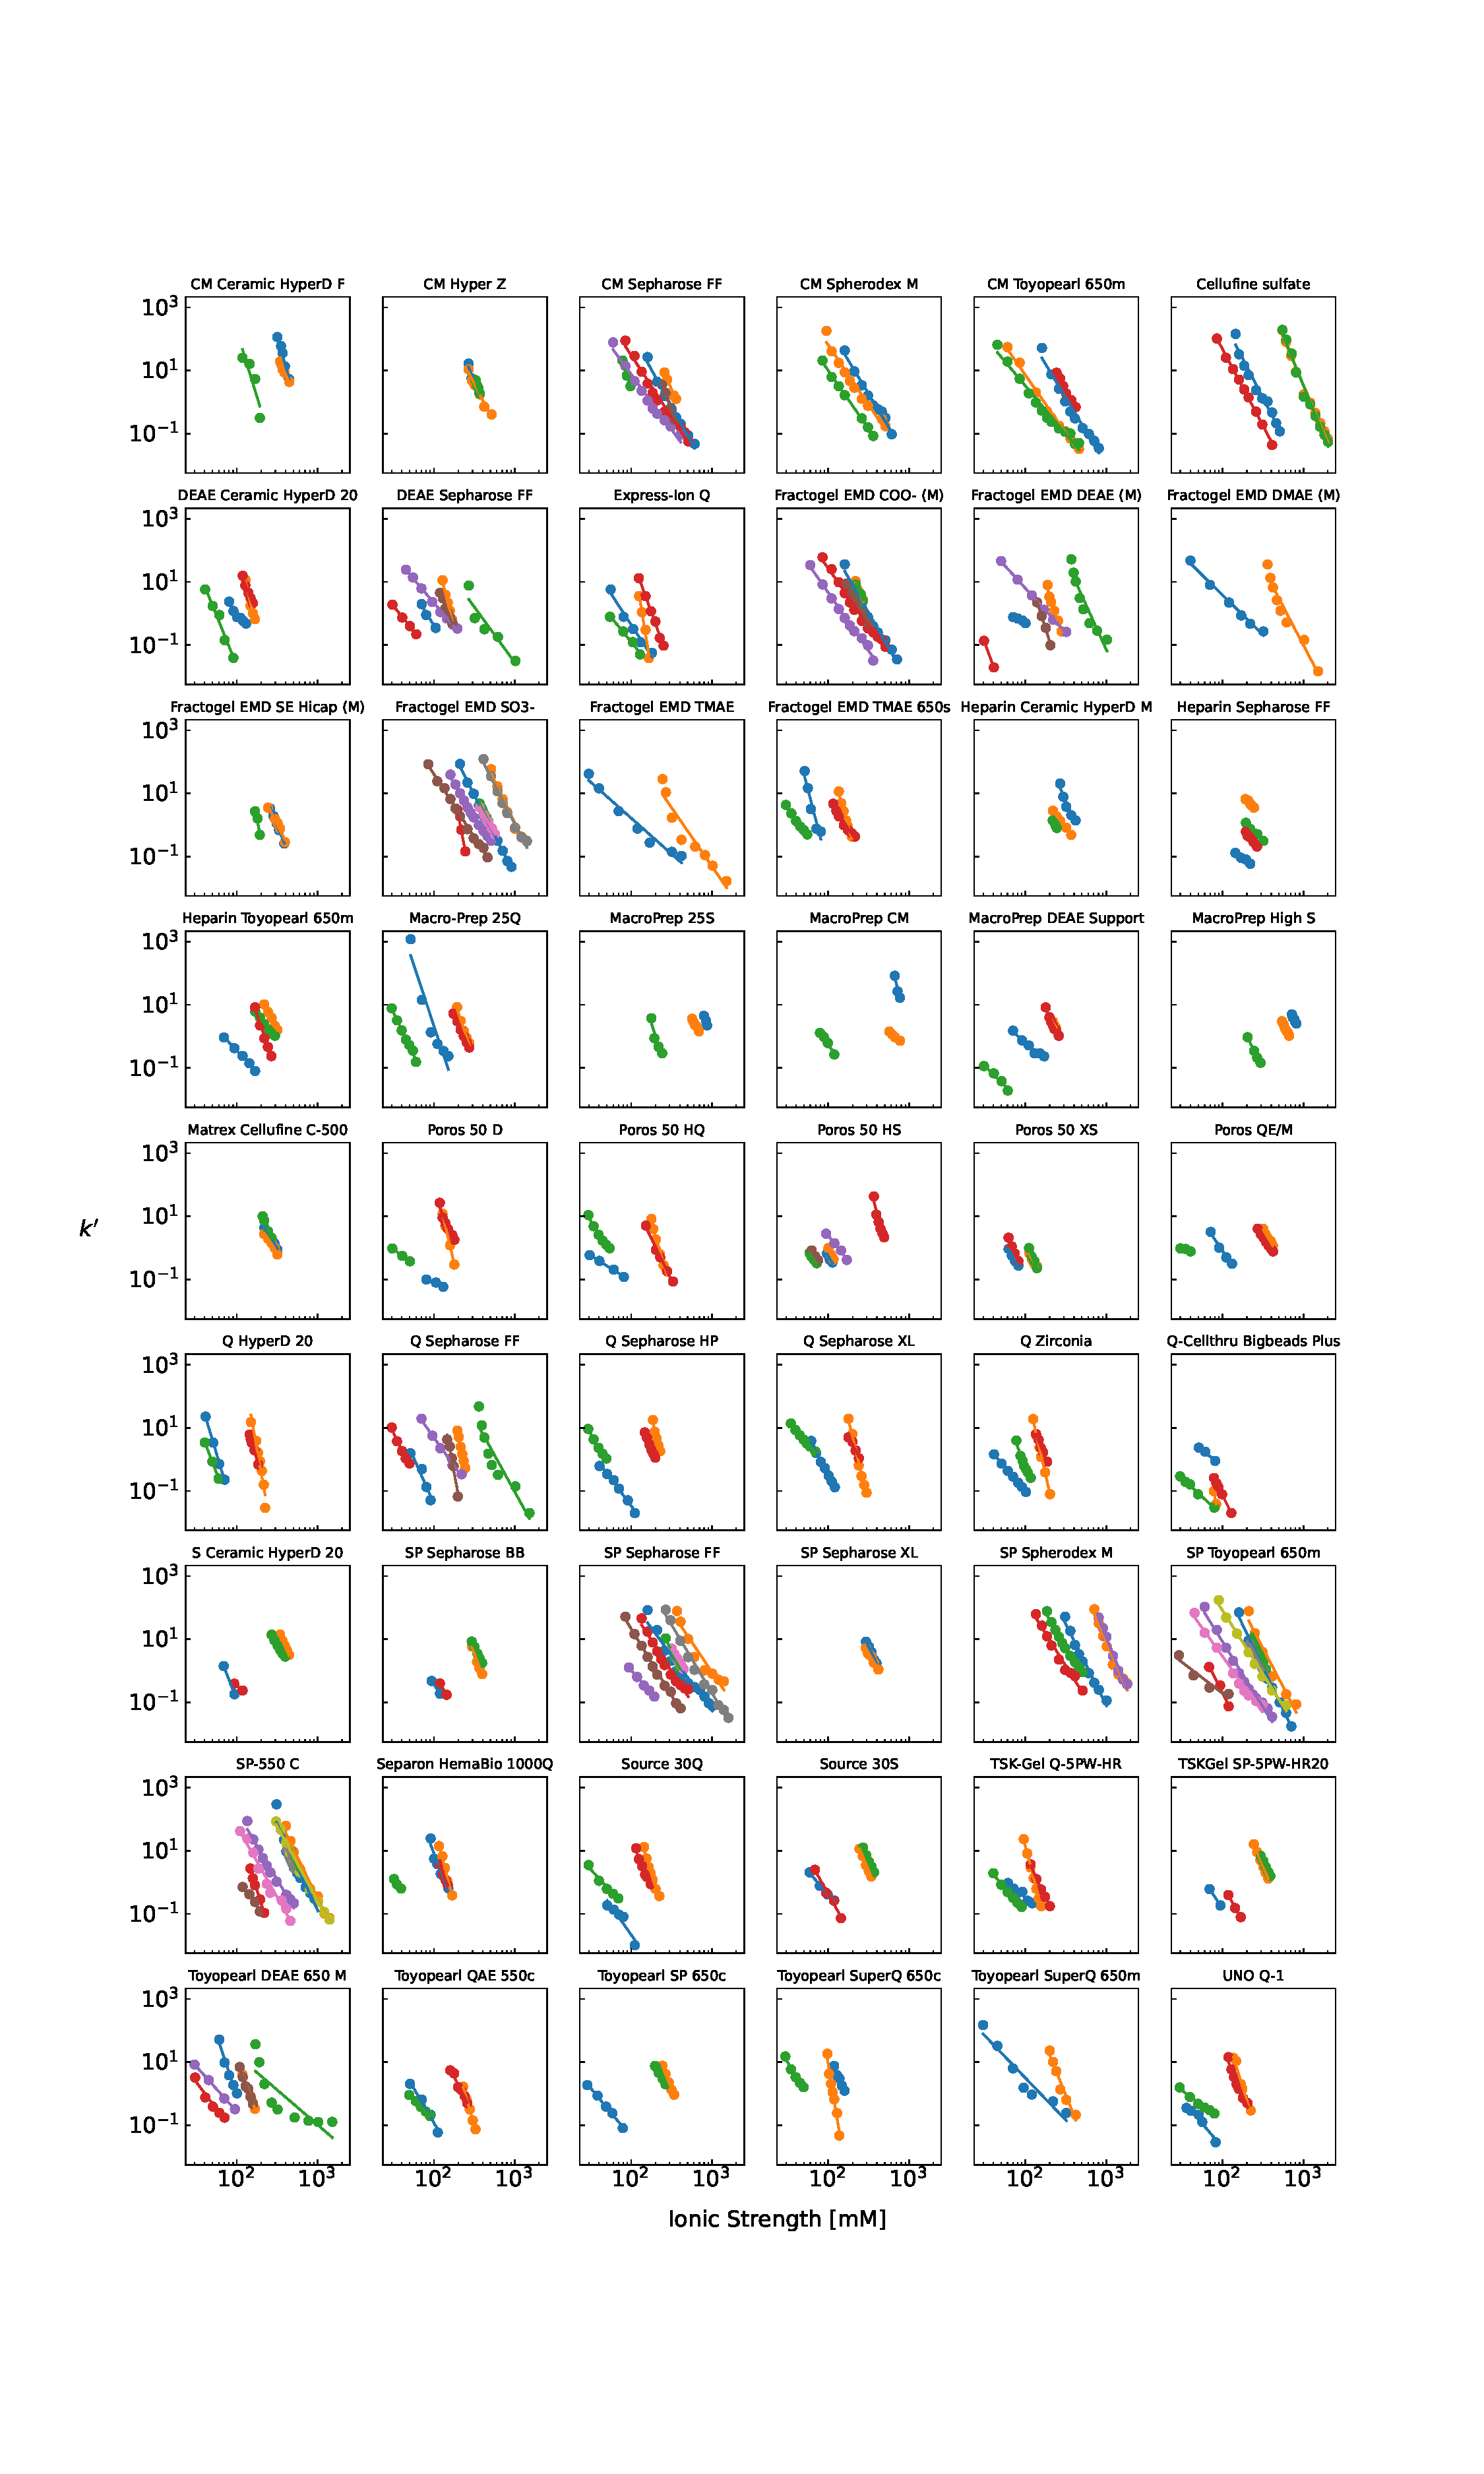
\includegraphics[width=1.15\textwidth]{figure_s2}}
    \vspace{-4cm}
    \caption{Isocratic $k'$ data that were consolidated from the literature. Each series represents a unique protein-pH-resin combination, and lines represent quasi-SDM fits to the data. These data, which are available in the \texttt{Supplementary\_table\_S2.xlsx} file, were acquired by digitizing plots (using the Engauge Digitizer software), which may introduce some error into the precise $k'$ values.}
    
    \label{fig:consolidated data}
\end{figure}


\begin{table}[h]
\caption{Simulation parameters.}
\label{tab:sim_params}
\begin{tabular}{l|l|l}
Variable                                & Figures 1, 2, and S1
                                        & Figure 3 \\
\hline
$L_{col}$ {[}cm{]}                       & 4.2 & 5.0 -- 20.0 \\
$r_p$ {[}$\mu$m{]}                       & 25.0 & 2.5 -- 100.0 \\
$\varepsilon_c$ {[} - {]}                & 0.49 & 0.49 \\
$\varepsilon_p$ {[} - {]}                & 0.40 & 0.40 \\
$u$, superficial velocity {[}cm/h{]}     & 300 & 100 -- 200 \\
$D_{ax}$ {[}m$^2$/s{]}                   & \num{1.25e-7} & Function of $u$\\
$k_{film}$ {[}m/s{]}                     & \num{1.0e-3} & \num{1.0e-3} \\
$D_p$ {[}m$^2$/s{]}                      & \num{1.0e-11} & \num{5.0e-12} -- \num{4.0e-11}\\
$a$ {[}m$^2$/s{]} (in $D_s = a K_{eq}^b$)  & \num{7.76e-12} & \num{1.66e-12} \\
$b$ {[} - {]} (in $D_s = a K_{eq}^b$)      & $-$1.54 & $-$0.24 \\
$K_{eq}$ {[} - {]}                       & \num{1.0e0} -- \num{1.0e4} & \num{1.0e0} -- \num{1.0e4} \\
$q_{max}$ {[}mg/ml column{]}             & 100 & 100 \\
$c_{load}$ {[}mg/ml{]}                   & \num{1.0e-3} -- \num{1.0e1} & \num{1.0e-3}
\end{tabular}
\end{table}

\end{document}
